\section{Problem V}
\textbf{solution}:\\
\begin{enumerate}
	\item \textit{Directed/Edges}\\
	$\Rightarrow$:\\
	If there are $k$ edge-disjoint paths from $s$ to $t$, then at the worst case, it will delete one edge on each of $k - 1$ paths from $k$ edge-disjoint paths we have. So, there is at least one path from $s$ to $t$ left after we delete $k - 1$ edges from $G$. So $t$ is still reachable from $s$. \\

	$\Leftarrow$:\\
	Let $(G, u, s, t)$ be a network with unit capacities $u = 1$ on each edge such that $t$ is reachable from $s$ even after deleting any $k - 1$ edges. This implies that the minimum capacity of an $s-t$ cut is at least $k$. By the Max-Flow-Min-Cut Theorem this flow can be decomposed into integral flows on $s-t$ paths. Since all capacities are 1 we must have at least $k$ edge-disjoint $s-t$ paths. 

	\item \textit{Directed/Vertices}\\
	$\Rightarrow$:\\
	If there are $k$ \textit{vertex-disjoint} paths from $s$ to $t$, then at the worst case, it will delete one vertex on each of $k - 1$ paths from $k$ vertex-disjoint paths we have. So, there is at least one path from $s$ to $t$ left after we delete $k - 1$ vertex from $G$. So $t$ is still reachable from $s$. \\

	$\Leftarrow$:\\
	\begin{figure}[h]
	\centering
	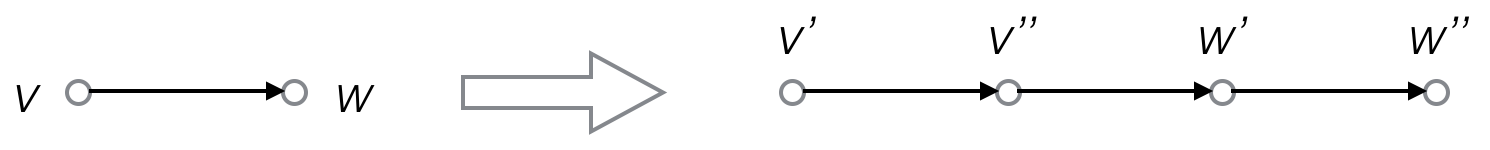
\includegraphics[scale=0.4]{hw4p5b}
	\caption{}
	\label{fig:p5b}
	\end{figure}
	We could replace each vertex $v$ of $G$ by two vertices $v'$ and $v''$ and an edge ($v'$, $v''$). Each edge ($v, w$) of $G$ is replaced by ($v'', w'$) and we assign capacity 1 with it as shown in Figure \ref{fig:p5b}. Any set of $k - 1$ edges in the new graph $G'$ whose deletion makes $t$ unreachable from $s$ implies a set of at most $k - 1$ vertices in $G$ whose deletion makes $t$ unreachable from $s$. Moreover, edge-disjoint $s''-t'-$paths in the new graph correspond to vertex-disjoint $s-t-$paths in the old one which could be transform into \textit{Directed/Edges} case. So according to the proof we have in \textit{Directed/Edges} case, we must have at least $k$ vertex-disjoint $s-t$ paths. 

	\item \textit{Undirected/Edges}\\
	$\Rightarrow$:\\
	Similar with the \textit{Directed/Edges} case, If there are $k$ edge-disjoint paths from $s$ to $t$, then at the worst case, it will delete one edge on each of $k - 1$ paths from $k$ edge-disjoint paths we have. So, there is at least one path from $s$ to $t$ left after we delete $k - 1$ edges from $G$. So $t$ is still reachable from $s$.\\

	$\Leftarrow$:\\
	\begin{figure}[h]
	\centering
	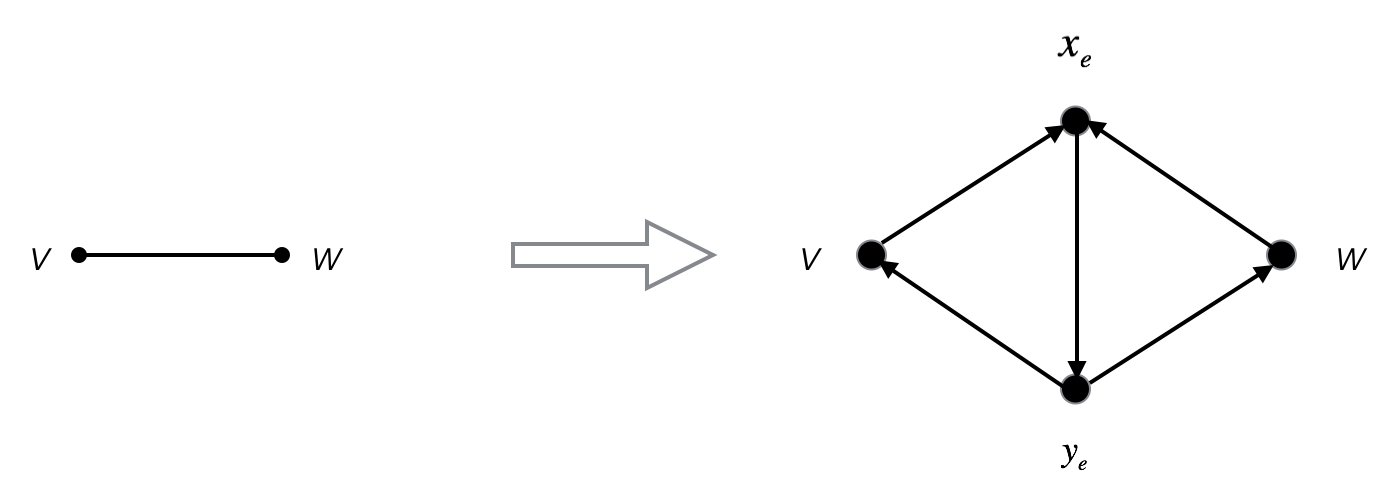
\includegraphics[scale=0.4]{hw4p5a}
	\caption{}
	\label{fig:p5a}
	\end{figure}
	Let $G$ be an undirected graph with two vertices $s$ and $t$ such that $t$ is reachable from $s$ even after deleting any $k - 1$ edges. This property obviously remains true if we replace each undirected edge $e = \left\{ v, w \right\}$  by five directed edges $(v, x_e), (w, x_e), (x_e, y_e), (y_e, v), (y_e, w)$ where $x_e$ and $y_e$ are new vertices as shown in Figure \ref{fig:p5a} with each edge has capacity 1. Now we have a digraph $G'$ and, by the proof of \textit{Directed/Edges} case, we must have at least $k$ edge-disjoint $s-t$ paths in $G'$. These can be easily transformed to $k$ edge-disjoint $s-t$ paths in $G$. 

	\item \textit{Undirected/Vertices}\\
	$\Rightarrow$:\\
	Similar with the \textit{Directed/Vertices} case, if there are $k$ \textit{vertex-disjoint} paths from $s$ to $t$, then at the worst case, it will delete one vertex on each of $k - 1$ paths from $k$ vertex-disjoint paths we have. So, there is at least one path from $s$ to $t$ left after we delete $k - 1$ vertex from $G$. So $t$ is still reachable from $s$. \\

	$\Leftarrow$:
	\begin{figure}[h]
	\centering
	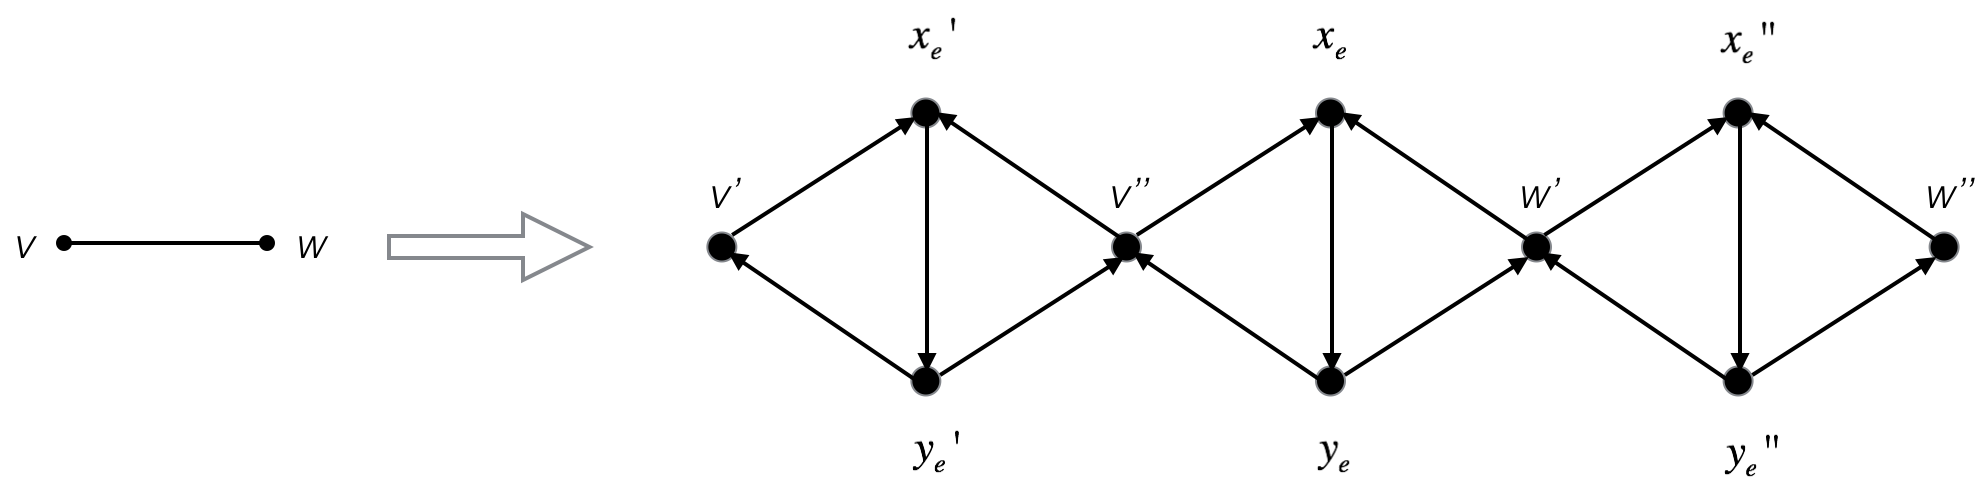
\includegraphics[scale=0.4]{hw4p5c}
	\caption{}
	\label{fig:p5c}
	\end{figure}
	Similar with what we did in \textit{Directed/Vertices} case, we could replace each vertex $v$ of $G$ by two vertices $v'$ and $v''$ and an edge ($v'$, $v''$). Then as what we did in \textit{Undirected/Edges} case, we replace each undirected edge $e = \left\{ v, w \right\}$  by five directed edges $(v, x_e), (w, x_e), (x_e, y_e), (y_e, v), (y_e, w)$ where $x_e$ and $y_e$ are new vertices and assign capacity 1 on each edge as shown in Figure \ref{fig:p5c}. Following the proof in \textit{Directed/Vertices} and \textit{Undirected/Edges} cases, we must have $k$ vertex-disjoint paths in $G$.
\end{enumerate}